\begin{figure}[!htb]
    \begin{centering}
        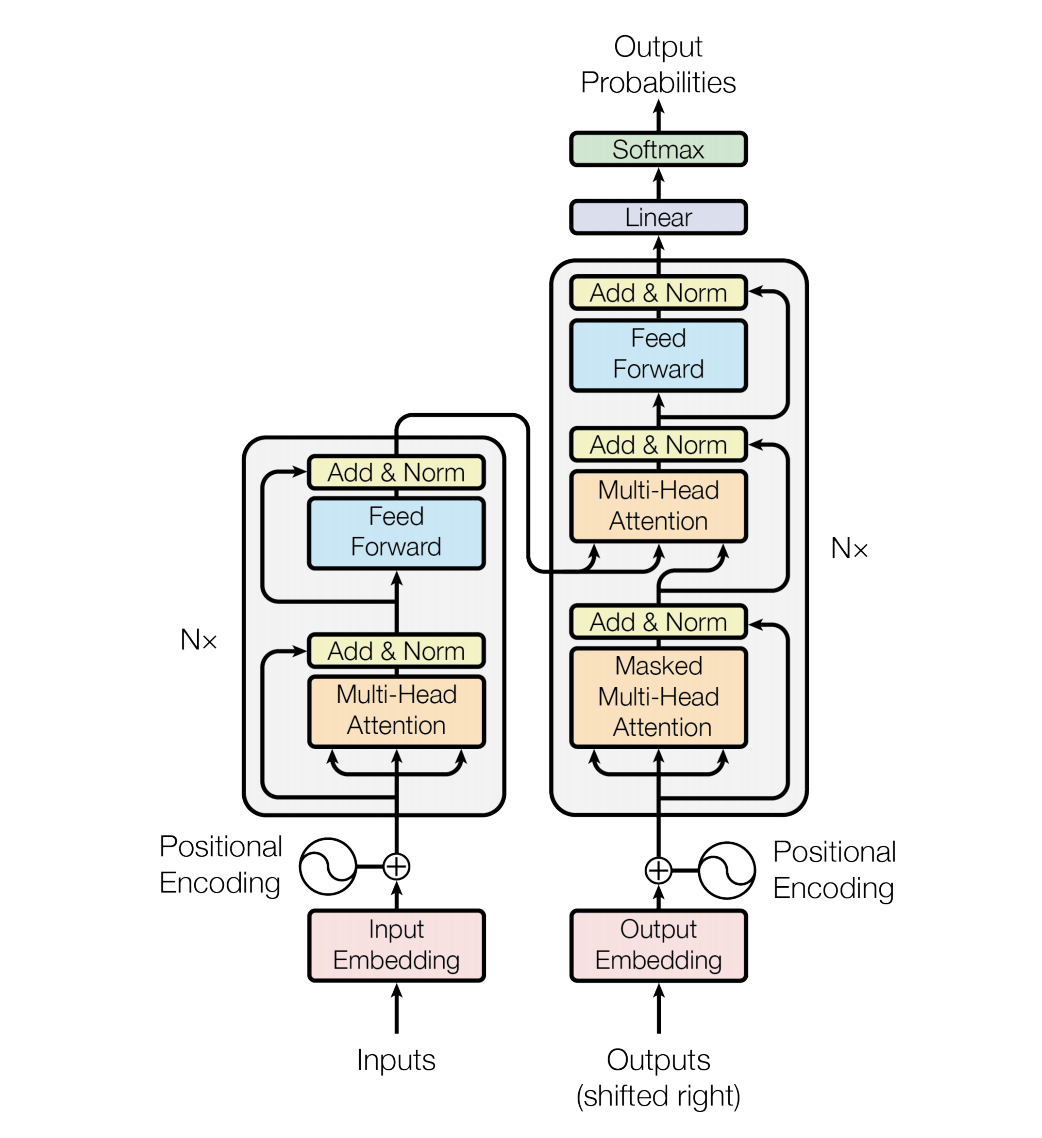
\includegraphics[height=0.5\textheight]{img/transformer}
        \caption[Original Transformer Architecture]{\textbf{Original Transformer Architecture.}
        The architecture was originally conceptualized for translation between languages.
        For that effect the text to translate (input) will be fully encoded to the embedding space, added to a positional encoding, and passed through alternating layers of self-attention and \gls{MLP} feed-forward layers with \gls{ReLU} activation, with residual connections and normalization after each.
        Output is generated autoregressively (generating each output token one-by-one, and append it to outputs to generate the next one), and has an additional layer of cross-attention to the input embedding.
        \Glspl{causal} are exclusively autoregressive decoder-only models.
        % The text to translate \textit{from} is the input, and the model will autoregressively (append selected output token to the outputs to generate the next output token until the full output has been generated) generate the full output.
        Image Source: \cite{vaswani_attention_2017}
        }
        \label{fig:transformer}
    \end{centering}
\end{figure}

% \begin{figure}[!htbp]
%     \begin{centering}
%         \subfloat[Runtime in minutes for correcting 25kb Matrix]
%         {\includegraphics[scale=0.9]{figures/results/runtime_25}} \\
%         % \caption[Correction time of 25kb]
%         % {\textbf{Runtime in minutes} for correcting the 25kb matrix.}
%         \subfloat[Runtime in minutes for correcting 50kb Matrix]
%         {\includegraphics[scale=0.9]{figures/results/runtime_50}}
%         \caption[Algorithm Runtimes]
%         {\textbf{Algorithm Runtimes} for correcting the different matrices. It
%         remains an open question why the difference between KR and RUST stays the
%         same, even though both ICE and RUST double their computation time. Smaller
%         is better.}
%         \label{fig:transformer}
%     \end{centering}
% \end{figure}
